\section{Scenarios}\label{sec:scenarios}
In the following subsection, we discuss a selection of scenario flows. This selection is based on the priority of the non-functional requirements and use cases or on interesting behaviour of the system they showcase. Note that only essential steps are depicted in the sequence diagrams: some minor details may be omitted for brevity.

\subsection{Av2 - PDSDBReplica fails}
Figure \ref{fig:seq_av2fail} describes how failure of a \ttt{PDSDBReplica} is detected and which actions are taken. If the \ttt{PDSReplicationManager} issues a query to a \ttt{PDSDBReplica} and it does not respond within four seconds, the \ttt{PDSDBReplica} is pinged. If that ping times out, the \ttt{PDSDBReplica} is perceived as having failed and a notification to the eDocs administrators is issued through the \ttt{CommunicationSubsystem}.

\begin{figure}[!htp]
    \centering
    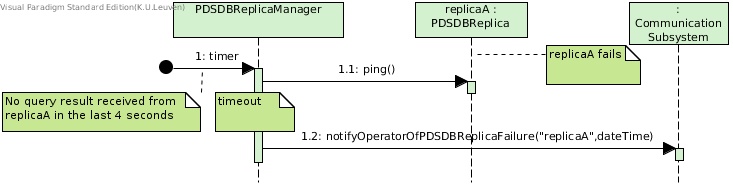
\includegraphics[width=0.8\textwidth]{figures/Av2 - PDSDBReplica fails.png}
    %\missingfigure[figwidth=0.8\textwidth]{Sequence diagram scenario 1}
    \caption{The system behavior for detection of \ttt{PDSDBReplica failure}.
        }\label{fig:seq_av2fail}
\end{figure}

\subsection{Av2 - PDSDBReplica back on-line}
Figure \ref{fig:seq_av2online} describes what happens when a previously failed replica comes back on-line. When the failed replica responds to a ping from the \ttt{PDSReplicationManager}, the \ttt{PDSReplicationManager} asks another replica for all documents that have been stored since failure was detected. Upon reception of these documents, they are all stored in the previously off-line replica. This way, that replica is brought back up to speed.

\begin{figure}[!htp]
    \centering
    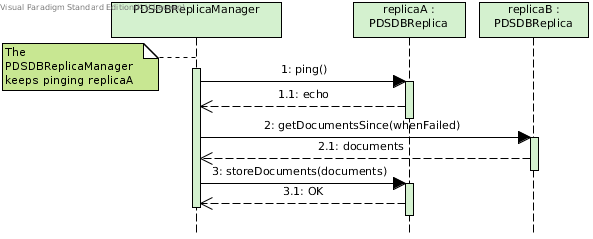
\includegraphics[width=0.7\textwidth]{figures/Av2 - PDSDBReplica back on-line.png}
    %\missingfigure[figwidth=0.8\textwidth]{Sequence diagram scenario 1}
    \caption{The system behavior for recovery from \ttt{PDSDBReplica} failure.
        }\label{fig:seq_av2online}
\end{figure}

\subsection{Av2b - Detecting PDSDB Failure}
Figure \ref{fig:seq_av2bfail} describes how failure of the \ttt{PDSDB} is detected and which actions are taken. If the \ttt{GeneratedDocumentHandler} sends a document for storage to the \ttt{PDSDB} and receives no acknowledgement within four seconds, the \ttt{PDSDB} is pinged. If that ping times out, the \ttt{PDSDB} is perceived as having failed and a notification to the eDocs administrators is issued through the \ttt{CommunicationSubsystem}. The Document IDs of all documents then arriving for the \ttt{PDSDB} are cached in the \ttt{PDSCache}, until the \ttt{PDSDB} comes back online.

\begin{figure}[!htp]
    \centering
    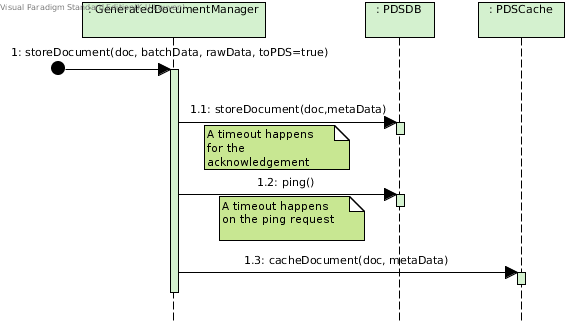
\includegraphics[width=0.65\textwidth]{figures/Av2b - Detecting PDSDB Failure.png}
    %\missingfigure[figwidth=0.8\textwidth]{Sequence diagram scenario 1}
    \caption{The system behavior for detection of \ttt{PDSDB failure}.
        }\label{fig:seq_av2bfail}
\end{figure}

\subsection{Av2b - PDSDB back on-line}
Figure \ref{fig:seq_av2bonline} describes what happens when the \ttt{PDSDB} comes back on-line. When it responds to a ping from the \ttt{GeneratedDocumentManager}, the latter will take notice of the fact that it has come back online. It will get all Document IDs out of the \ttt{PDSCache} and retrieves the corresponding documents and metadata from the \ttt{DocumentDB}. It then proceeds to store them in the \ttt{PDSDB}.

\begin{figure}[!htp]
    \centering
    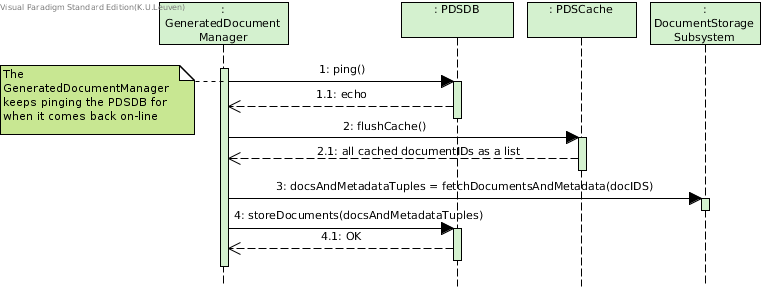
\includegraphics[width=0.7\textwidth]{figures/Av2b - PDSDB back on-line.png}
    %\missingfigure[figwidth=0.8\textwidth]{Sequence diagram scenario 1}
    \caption{The system behavior for recovery from \ttt{PDSDB failure}.
        }\label{fig:seq_av2bonline}
\end{figure}


\subsection{Av3 - Zoomit failure}
Figure \ref{fig:seq_av2bfail} describes how failure of the external \ttt{Zoomit} service is detected and which actions are taken. When the \ttt{ZoomitDeliveryHandler} sends a document to the \ttt{Zoomit} service and does not receive an acknowledgement, it caches the \ttt{documentID} and accompanying \ttt{DeliveryMetaData} in the \ttt{ZoomitDocumentLinkCache}. When the failure is detected for the first time, an exponential backoff timer is started. Every time the timer signals, all documentIDs and metadata are popped from the \ttt{Cache} and a resend is attempted after retrieving the actual documents from the \ttt{DocumentStorageSubsystem}. Every failed delivery goes back into the \ttt{Cache}. After the limit of exponential backoff iterations is reached for a number of different documents (conform \emph{Av3}, a notice is sent to the eDocs Administrator.

\begin{figure}[!htp]
    \centering
    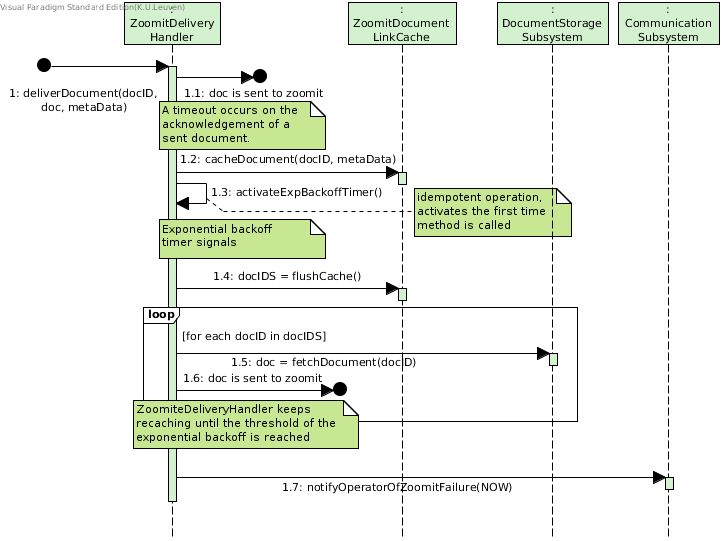
\includegraphics[width=0.7\textwidth]{figures/Av3 - Zoomit failure.png}
    %\missingfigure[figwidth=0.8\textwidth]{Sequence diagram scenario 1}
    \caption{The system behavior for detection of \ttt{Zoomit failure}.
        }\label{fig:seq_av3fail}
\end{figure}



\subsection{UC1 - Login}\label{sec:seq_uc1}
Figure \ref{fig:seq_uc1} shows the steps taken to log in a user. Logging in consists of trying to create a session using the credentials supplied by the user. The first concern is verifying the user's credentials, which is the responsibility of the \ttt{AuthenticationManager}. Depending on the type of login request, the login details matching the supplied username are fetched from either the \ttt{RegisteredRecipientDatabase}, \ttt{COAdminDatabase} or \ttt{eDocsAdminDatabase}. After the login details have been received, the supplied credentials and the login details are compared. If successful, the \ttt{AuthenticationManager} returns a login token, upon which the session can be created. If unsuccessful, an AuthException is thrown and it is indicated to the user he supplied invalid credentials.

\begin{figure}[!htp]
    \centering
    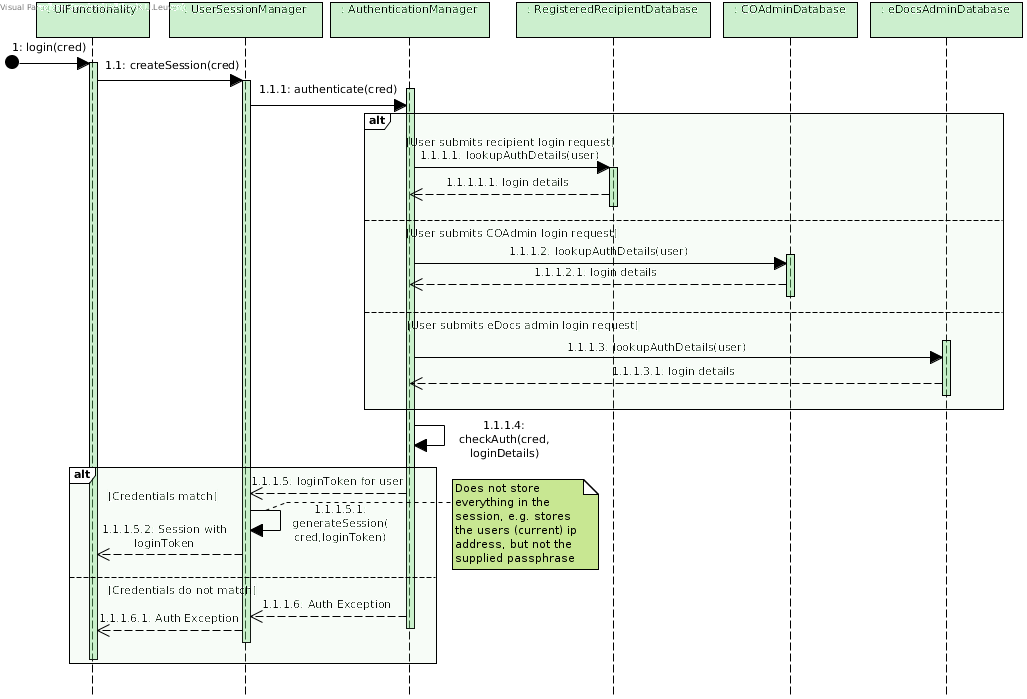
\includegraphics[width=\textwidth]{figures/UC1 - Login.png}
    %\missingfigure[figwidth=0.8\textwidth]{Sequence diagram scenario 1}
    \caption{The system behavior for Use Case 1.
        }\label{fig:seq_uc1}
\end{figure}

\subsection{UC3 - Initiate document processing}\todo{fix sequence diagram: submitJobs}
Figure \ref{fig:seq_uc3} shows the steps taken to submit raw data, with some minor details omitted for brevity. First, the data submitter sends details about the batch they plan to submit. These batch details are first verified by the \ttt{RawDataVerifier} and an exception is thrown when something is out of order (refer to section \ref{sec:rawdataverifier} for details about when the exception is thrown). When the batch details have been successfully verified, the submitter uploads the batch. Now, the integrity of the batch is verified and thereafter all individual entries. If any individual entries fail verification, an exception is thrown and it is indicated which entries failed and why (again, refer to section \ref{sec:rawdataverifier} as to what exactly is verified). All entries that passed verification are now supplied to the \ttt{JobGenerator}, where \ttt{Job} objects are generated and finally passed to the \ttt{JobSubmitter}, which stores them. The \ttt{Job}s are also passed to the \ttt{Scheduler} so that document generation may begin. 

\begin{figure}[!htp]
    \centering
    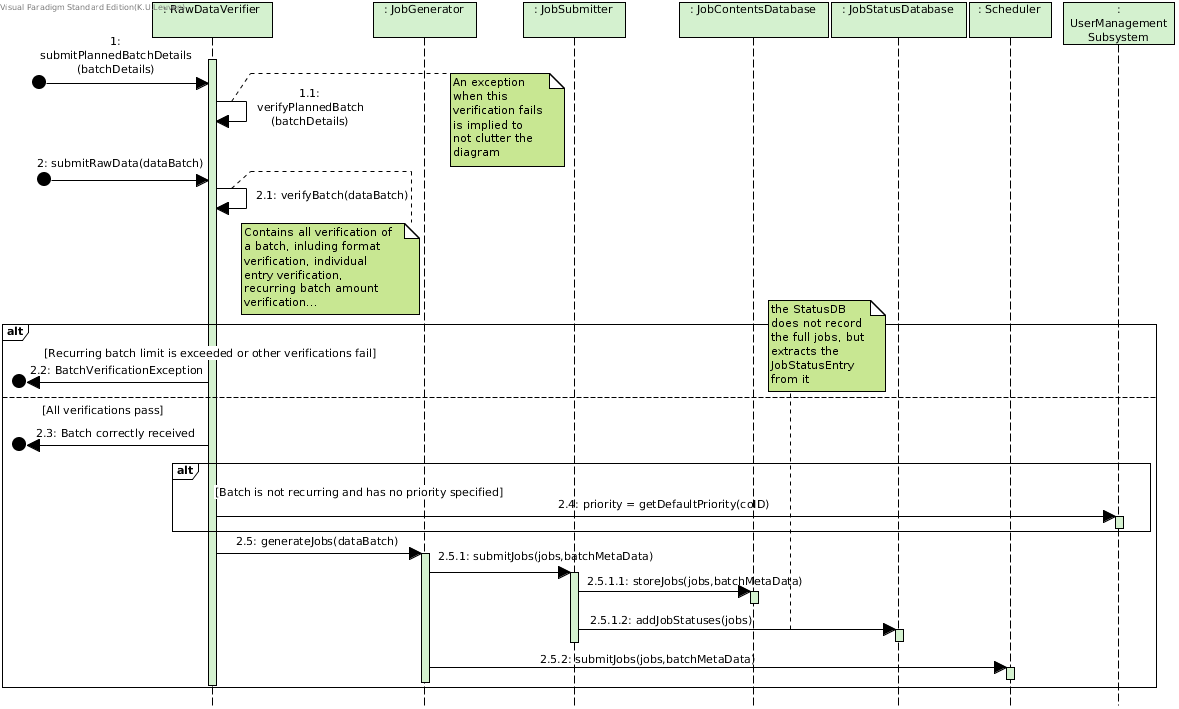
\includegraphics[width=\textwidth]{figures/UC3 - Initiate document processing.png}
    %\missingfigure[figwidth=0.8\textwidth]{Sequence diagram scenario 1}
    \caption{The system behavior for Use Case 3.
        }\label{fig:seq_uc3}
\end{figure}

\subsection{UC4/5 - Process Jobs}
Figures \ref{fig:seq_uc45_1} and \ref{fig:seq_uc45_2} show how documents are generated. One way or the other, the \ttt{Generator} receives a new batch to work on. It then asks the \ttt{Completer} to fetch the raw data and meta-data, which asks the \ttt{JobStorageSystem} in turn. We assume here that it concerns an invoice, therefore the key is needed. The \ttt{KeyCache} is asked for it, which asks the \ttt{UserManagementSubsystem}, if necessary. Next, the \ttt{Completer} asks the \ttt{TemplateCache} for the template. The \ttt{UserManagementSubsytem} again provides the template, if necessary. With all that data collected, the \ttt{Completer} finally gives it all to the \ttt{Generator}. The \ttt{Generator} then generates the document, handing it to the \ttt{GeneratedDocumentHandler} for storage and delivery. If something is wrong with the raw data (e.g. insufficient information with which to fill out the template), then the \ttt{CommunicationSubsystem} is notified of the error, instead.

\begin{figure}[!htp]
    \centering
    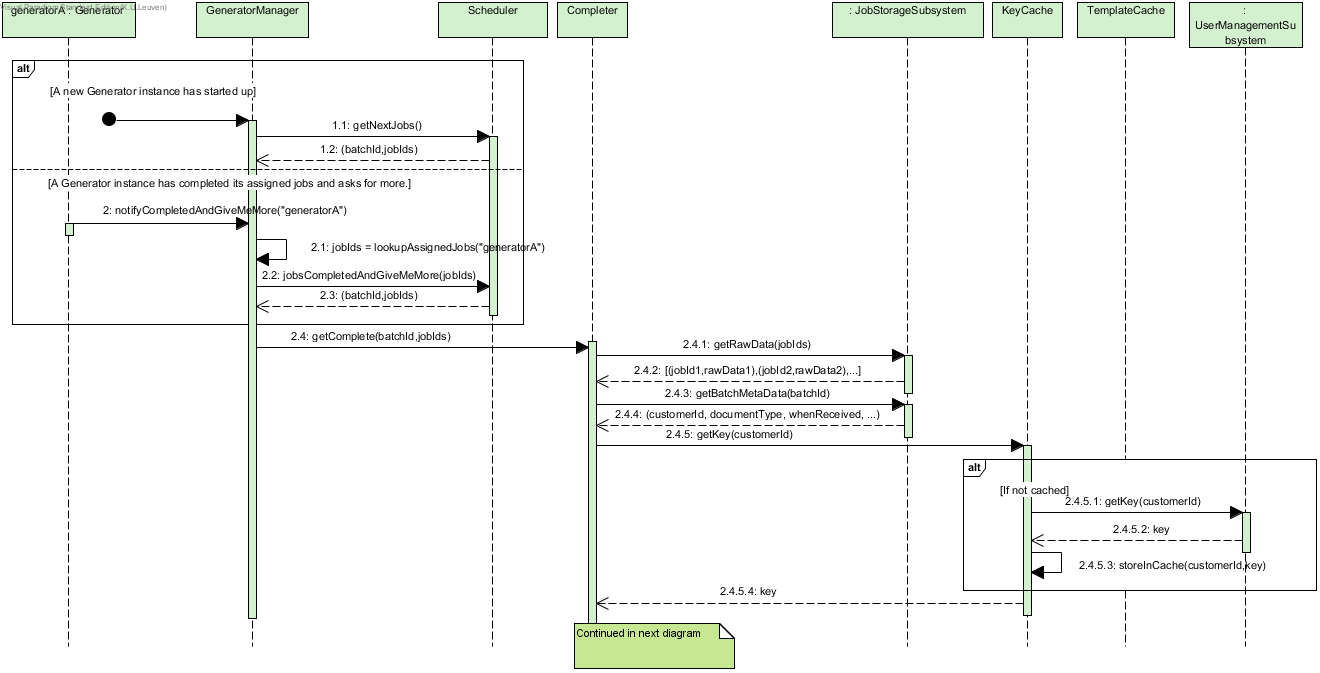
\includegraphics[width=\textwidth]{figures/UC4_5 - ProcessJobs1.png}
    %\missingfigure[figwidth=0.8\textwidth]{Sequence diagram scenario 1}
    \caption{The system behavior for Use Cases 4 and 5.
        }\label{fig:seq_uc45_1}
\end{figure}

\begin{figure}[!htp]
    \centering
    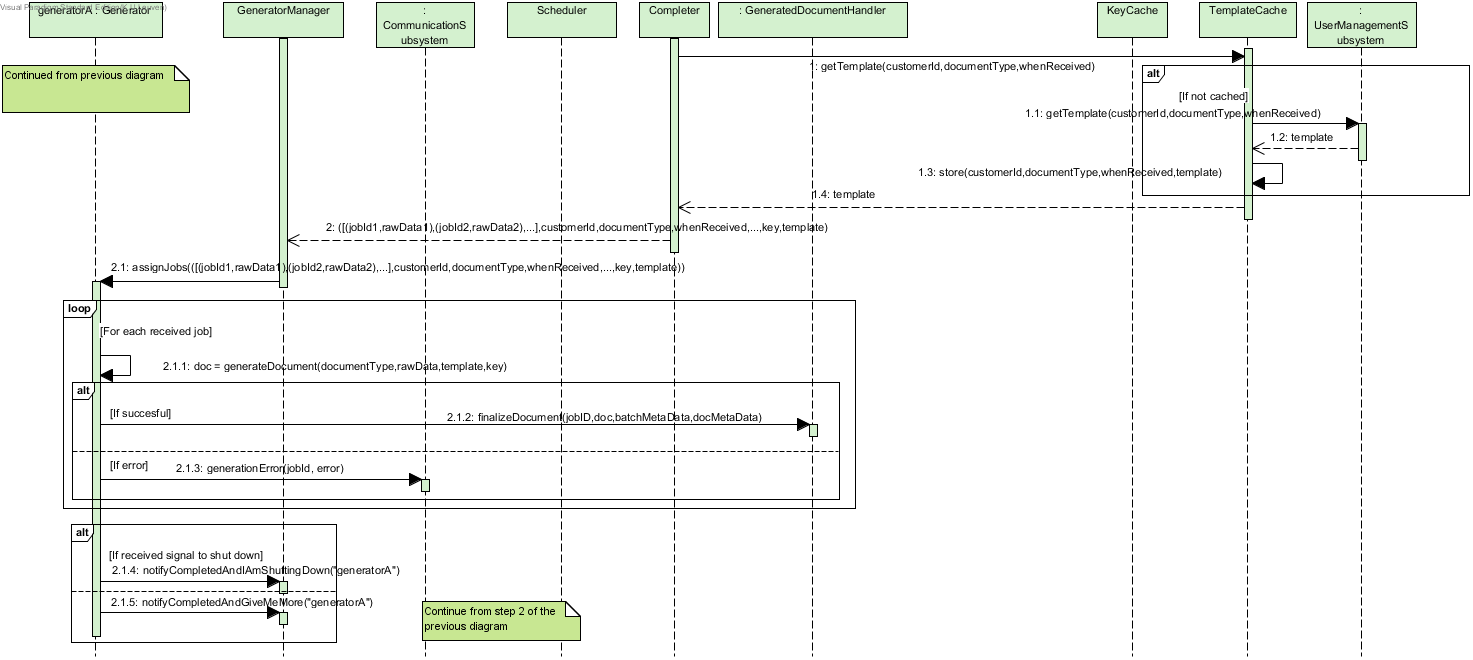
\includegraphics[width=\textwidth]{figures/UC4_5 - ProcessJobs2.png}
    %\missingfigure[figwidth=0.8\textwidth]{Sequence diagram scenario 1}
    \caption{Continuation of system behavior for Use Cases 4 and 5.
        }\label{fig:seq_uc45_2}
\end{figure}

\subsection{UC6 - Deliver document via e-mail}
Figure \ref{fig:seq_uc6} shows the steps undertaken in order to deliver a document via e-mail. First, it is determined if the Customer Organization has activated receipt tracking. Then, the \ttt{GeneratedDocumentHandler} generates a \ttt{DeliveryMetaData} object from the \ttt{BatchMetaData} and \ttt{RawDataMetaData} provided (this includes a check whether the supplied e-mail address is present in the \ttt{UserManagementSubsytem}, in which case it is indicated the document should be delivered via Personal Document Store instead). After this, it is passed on to the \ttt{DocumentDistributor}, which analyses the \ttt{DeliveryMetaData} object and hands it to the \ttt{EmailDeliveryChannel} when it sees it should be delivered via e-mail. Depending on whether receipt tracking is enabled or not, a download link is requests from the  \ttt{LookupLinkCodec}. Now, the e-mail is composed and handed to the \ttt{CommunicationSubsystem} for submission to the e-mail provider.

\begin{figure}[!htp]
    \centering
    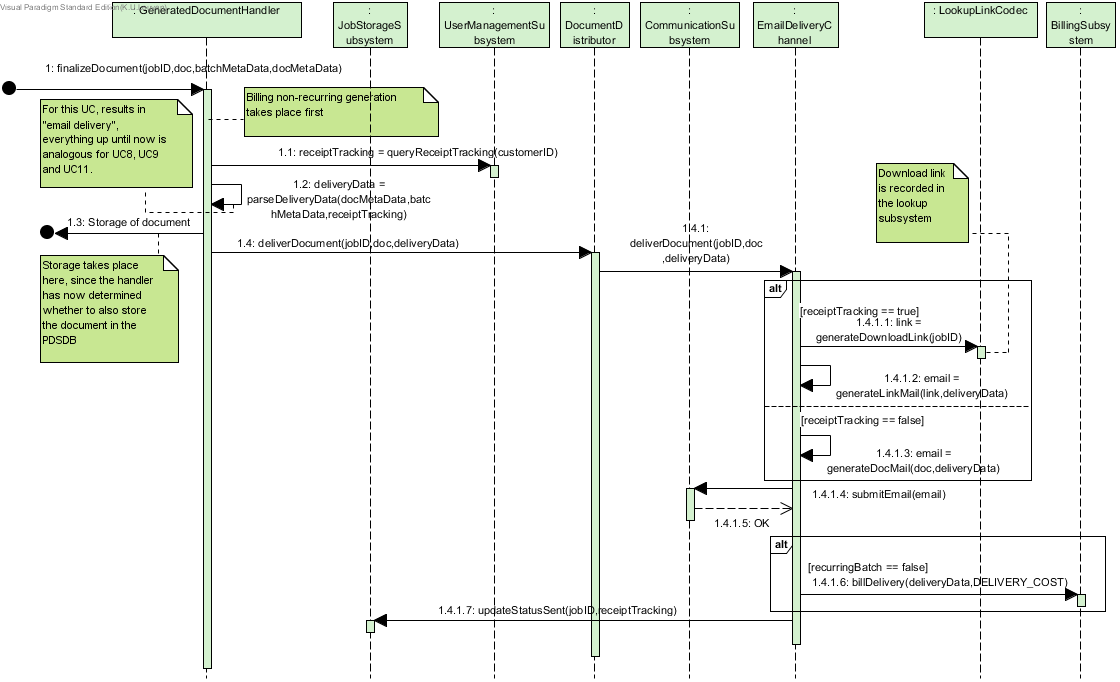
\includegraphics[width=\textwidth]{figures/UC6 - Deliver document via e-mail.png}
    %\missingfigure[figwidth=0.8\textwidth]{Sequence diagram scenario 1}
    \caption{The system behavior for Use Case 6.
        }\label{fig:seq_uc6}
\end{figure}

\subsection{UC7 - Signal e-mail delivery failure}
Figure \ref{fig:seq_uc7} shows the steps undertaken when a signal is received that e-mail delivery has failed. First, the \ttt{ExternalNotificationAcceptor} extracts the \ttt{JobID} from the e-mail (assumed present in the filename if receipt tracking was not activated; may require an extra call to the \ttt{LookupLinkCodec} if receipt tracking was activated and thus a download link is received). Now, the \ttt{JobStorageSubsytem} is told to update the status of the document to reflect that delivery has failed, whereafter the \ttt{CustomerOrganizationID} and the \ttt{DocumentType} are fetched. Based on those details, the e-mail address of the appropriate Customer Administrator is retrieved from the \ttt{UserManagementSubsystem} and an e-mail sent to this address.

\begin{figure}[!htp]
    \centering
    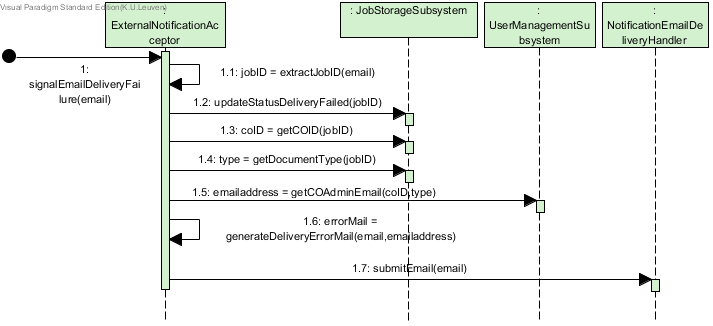
\includegraphics[width=0.7\textwidth]{figures/UC7 - Signal e-mail delivery failure.png}
    %\missingfigure[figwidth=0.8\textwidth]{Sequence diagram scenario 1}
    \caption{The system behavior for Use Case 7.
        }\label{fig:seq_uc7}
\end{figure}

\subsection{UC10 - Zoomit Receipt Confirmation}
Figure \ref{fig:seq_uc10} shows the steps undertaken when Zoomit confirms receipt of a document. The \ttt{JobID} is extracted from the notification from Zoomit (we assume that the name of the document, of which the \ttt{JobID} is a part, is present). Afterwards, the \ttt{JobStorageSystem} is notified that the specified document has been received.

\begin{figure}[!htp]
    \centering
    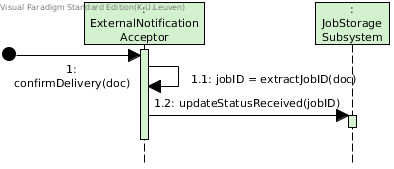
\includegraphics[width=0.4\textwidth]{figures/UC10 - Zoomit Receipt Confirmation.png}
    %\missingfigure[figwidth=0.8\textwidth]{Sequence diagram scenario 1}
    \caption{The system behavior for Use Case 10.
        }\label{fig:seq_uc10}
\end{figure}

\subsection{UC11a - Storing a document in the PDS} \todo{replace PDSContentManager with DocumentStorageHandler in sequence diagram}
Figure \ref{fig:seq_uc11a} shows the steps undertaken in order to store a document in the Personal Document Store. The sequence diagram as shown is fairly straightforward.

\begin{figure}[!htp]
    \centering
    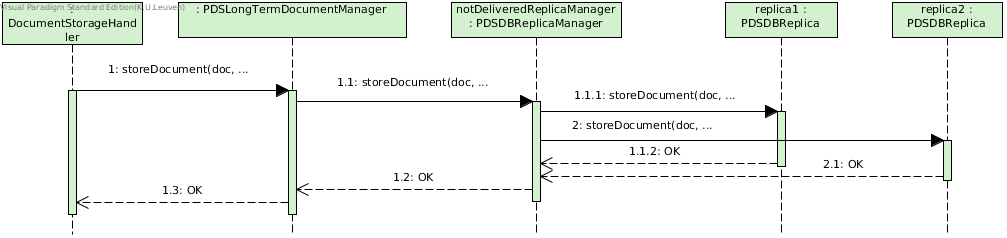
\includegraphics[width=\textwidth]{figures/UC11a - Storing a document in the PDS.png}
    %\missingfigure[figwidth=0.8\textwidth]{Sequence diagram scenario 1}
    \caption{The system behavior for storing documents in the Personal Document Store.
        }\label{fig:seq_uc11a}
\end{figure}

\subsection{UC14 - Consult document in PDS}
Figure \ref{fig:seq_uc14} shows the steps undertaken when consulting a document in the Personal Document Store. The \ttt{PDSLookupModule} either receives that request in the context of the user selecting a document in the web interface, in which case it can just forward the request to the \ttt{DocumentStorageSubsystem}, or it is supplied with a link. First, the link is handed to the  \ttt{LookupLinkCodec}, which answers with a \ttt{RecipientID} and \ttt{JobID}. In case the received \ttt{RecipientID} does not match with the user's \ttt{RecipientID}, an exception is thrown and directly propagated to the user's software via the \ttt{UserSession}. If they do match, the \ttt{LoadBalancer} is first asked for permission to execute the request. If granted, the request is now forwarded to the \ttt{DocumentStorageSubsystem} via an asynchronous call (the \ttt{DocumentStorageSubsystem} is expected to answer directly to the \ttt{UserSession}). Afterwards, if receipt tracking is enabled and the status of the document was not set to Received earlier, the \ttt{JobStorageSubsystem} is now directed to set the status to Received.

\begin{figure}[!htp]
    \centering
    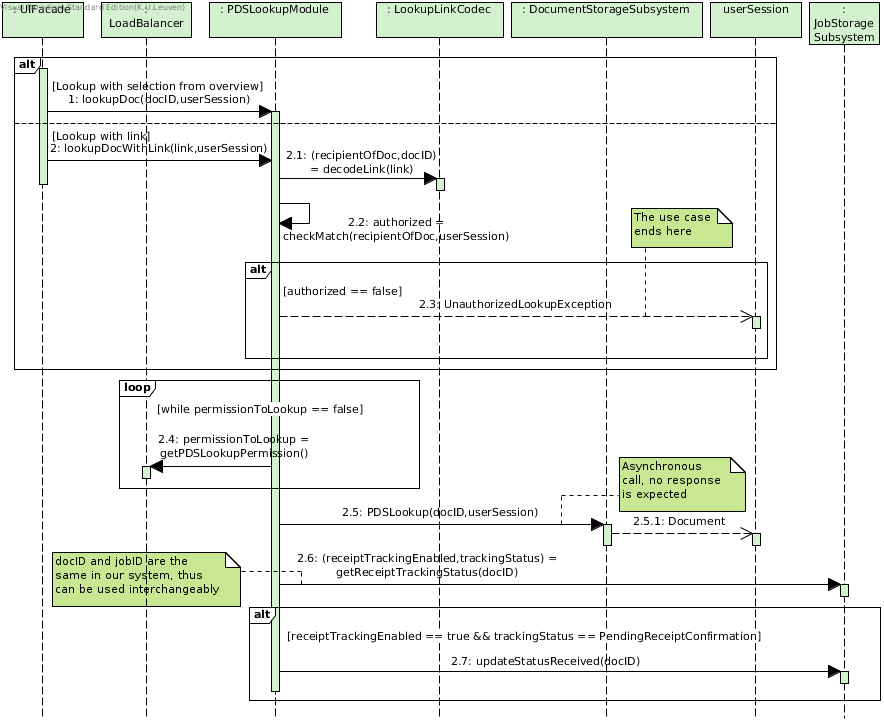
\includegraphics[width=\textwidth]{figures/UC14 - Consult document in PDS.png}
    %\missingfigure[figwidth=0.8\textwidth]{Sequence diagram scenario 1}
    \caption{The system behavior for Use Case 14.
        }\label{fig:seq_uc14}
\end{figure}

\subsection{UC15 - Download document via unique link}
Figure \ref{fig:seq_uc15} shows the steps undertaken if a Recipient looks up document via download link. First, it is checked whether the link is present in the \ttt{DownloadLinkCatalogue}. If not, the link has either expired or never existed in the first place. It is invalid either way, and this is reflected by throwing an exception. If it is valid, the \ttt{LookupLinkCodec} decodes the link and returns the \ttt{JobID}. Now, the \ttt{LoadBalancer} is first asked for permission. If granted, the request is forwarded to the \ttt{DocumentStorageSubsystem} via an asynchronous call. Immediately afterwards, the \ttt{DownloadLinkCatalogue} is notified of the fact that the link has been visited in order to ensure that the expiration of this link will not result in an erroneous notification to the Customer Organization that it has expired without the Recipient ever having viewed the document.

\begin{figure}[!htp]
    \centering
    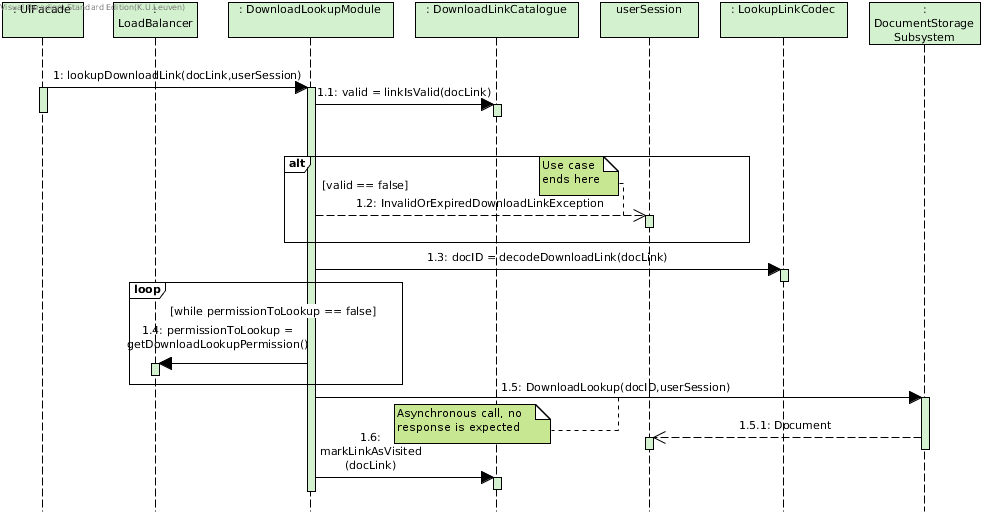
\includegraphics[width=\textwidth]{figures/UC15 - Download document via unique link.png}
    %\missingfigure[figwidth=0.8\textwidth]{Sequence diagram scenario 1}
    \caption{The system behavior for the first scenario.
        }\label{fig:seq_uc15}
\end{figure}

\subsection{UC16 - Register to PDS}
Figure \ref{fig:seq_uc16} shows the steps undertaken in order to register a Recipient to the Personal Document Store. First, it is determined whether the registration details supplied by the user are complete (e.g. e-mail address and full name present) and whether an account already exists with that e-mail address. If everything is in order, the Recipient is registered in the \ttt{RegisteredRecipientDatabase}. Afterwards, the \ttt{DocumentStorageHandler} is told to copy all documents in \ttt{DocumentDB} addressed to the newly registered Recipient to the \ttt{PDSDB}. When completed, the request to register is acknowledged and the Recipient is logged in (refer to section \ref{sec:seq_uc1})

\begin{figure}[!htp]
    \centering
    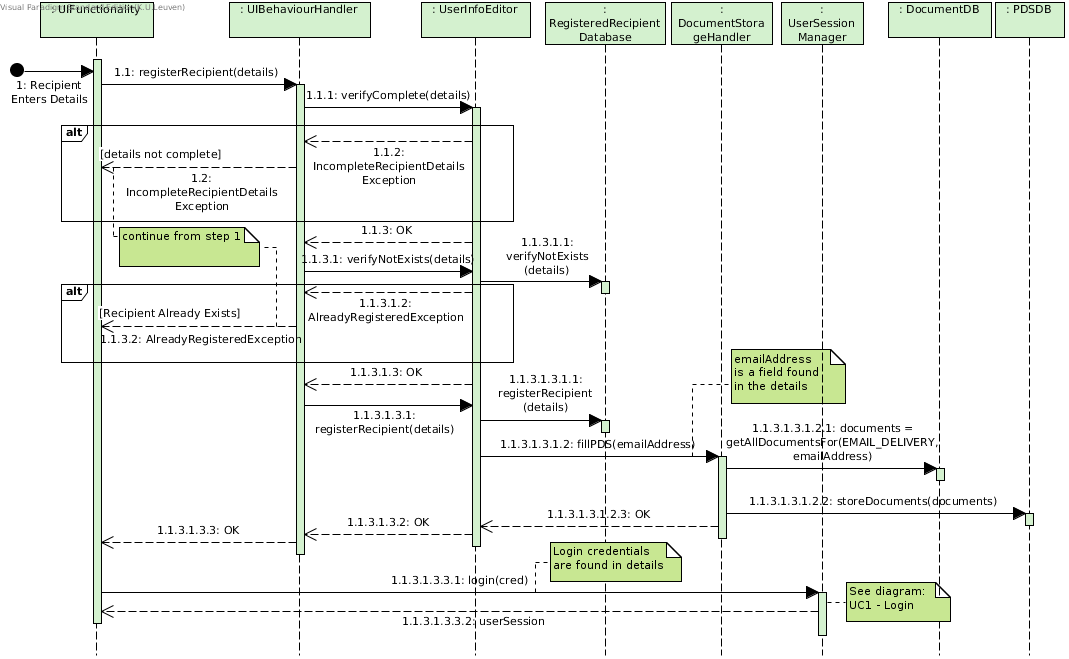
\includegraphics[width=\textwidth]{figures/UC16 - Register to PDS.png}
    %\missingfigure[figwidth=0.8\textwidth]{Sequence diagram scenario 1}
    \caption{The system behavior for Use Case 16.
        }\label{fig:seq_uc16}
\end{figure}

\subsection{UC21 - Consult Status of all Document Processing Jobs}
Figure \ref{fig:seq_uc21} shows the steps undertaken when a Customer Administrator requests an overview of all of that Customer Organization's jobs. The request is forwarded directly to the \ttt{JobStatusDatabase}, where the \ttt{CustomerOrganizationID} is extracted from the \ttt{UserSession} and the statuses of all jobs belonging to that Customer Organization are looked up. When completed, the overview is directly forwarded to the user's software via the \ttt{UserSession}.

\begin{figure}[!htp]
    \centering
    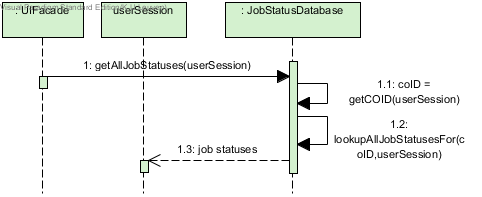
\includegraphics[width=0.5\textwidth]{figures/UC21 - Consult Status of all Document Processing Jobs.png}
    %\missingfigure[figwidth=0.8\textwidth]{Sequence diagram scenario 1}
    \caption{The system behavior for Use Case 21.
        }\label{fig:seq_uc21}
\end{figure}

\subsection{UC22 - Notify customer administrator}
Figure \ref{fig:seq_uc22} shows the steps undertaken in order to notify a Customer Administrator. Either a prepared e-mail is submitted, in which case it is forwarded to an external e-mail provider, or a message and \ttt{JobID} are provided. If the latter, then the \ttt{CustomerOrganizationID} is extracted from the \ttt{JobID} (a \ttt{JobID} is a combination of the \ttt{CustomerOrganizationID} and the identifier unique within the set of documents of that Customer Organization). Then, the \ttt{JobStorageSubsystem} is asked for the document type of the document corresponding to the \ttt{JobID}. Afterwards, the e-mail address of the appropriate Customer Organization is retrieved from the \ttt{UserManagamentSubsystem} based on the \ttt{CustomerOrganizationID} and document type. Now, an e-mail message can be composed that contains the message and is addressed to the correct e-mail address. Finally, the e-mail is sent to an e-mail provider.

\begin{figure}[!htp]
    \centering
    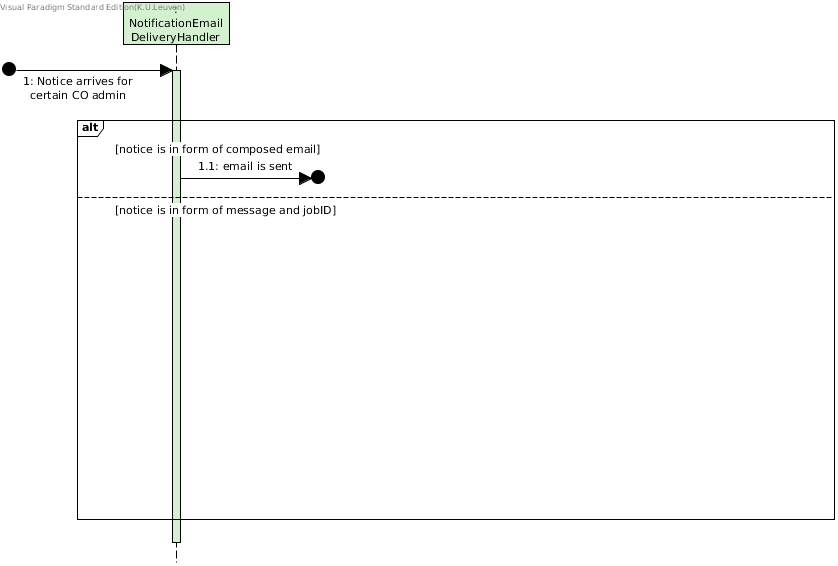
\includegraphics[width=0.6\textwidth]{figures/UC22 - Notify CO administrator.png}
    %\missingfigure[figwidth=0.8\textwidth]{Sequence diagram scenario 1}
    \caption{The system behavior for Use Case 22.
        }\label{fig:seq_uc22}
\end{figure}

\subsection{UC22', Av1a, Av2a - Notify eDocs administrator}
%TODO write scenario

\begin{figure}[!htp]
    \centering
    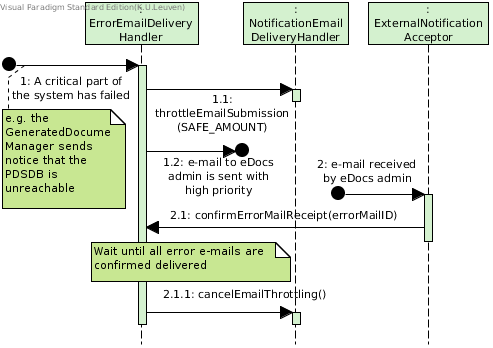
\includegraphics[width=0.6\textwidth]{figures/Av1a_2a UC22' - Notify eDocs Admin.png}
    %\missingfigure[figwidth=0.8\textwidth]{Sequence diagram scenario 1}
    \caption{The system behavior for Use Case 22', \emph{Av1a} and \emph{Av2a}.
        }\label{fig:seq_uc22'}
\end{figure}
